\documentclass[11pt, oneside]{article} 
\usepackage{geometry}
\geometry{letterpaper} 
\usepackage{graphicx}
	
\usepackage{amssymb}
\usepackage{amsmath}
\usepackage{parskip}
\usepackage{color}
\usepackage{hyperref}

\graphicspath{{/Users/telliott_admin/Dropbox/Tex/png/}}
% \begin{center} 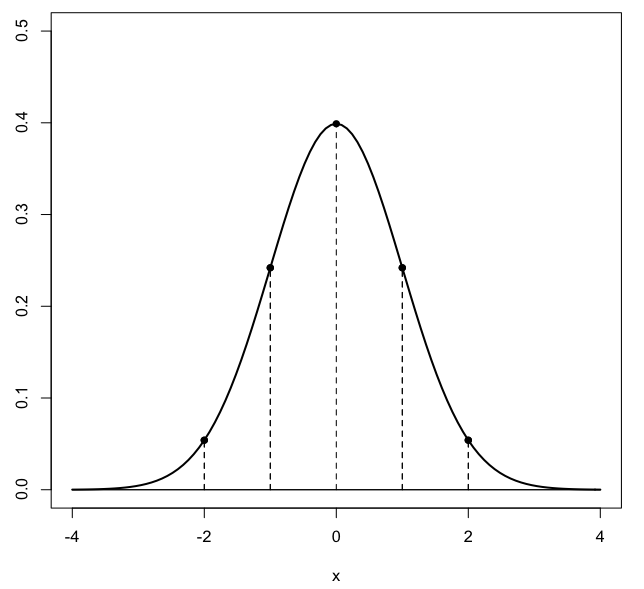
\includegraphics [scale=0.4] {gauss3.png} \end{center}

%break
\title{Rotation of conic sections}
\date{}

\begin{document}
\maketitle
\Large
Yet another thing that can happen to make life complicated is rotation.

Consider the rotated parabola.  You are probably used to seeing examples where it opens to the right or left.  These are obtained by having an equation like
\[ a(y-k)^2 = (x-h)  \]
with $x = g(y)$

Then, the easiest thing to do is to switch $x$ for $y$, solve the problem, and switch back at the end.

But it is also possible to rotate through a different angle, like $45^\circ$.  What happens then?  Well, basically we replace $x$ and $y$ by $u$ and $v$ with
\[ x = u \cos \theta - v \sin \theta \]
\[ y = u \sin \theta + v \cos \theta \]

(I derived these  \hyperref[sec:Geometric_rotation]{\textbf{here}}).
For $45^\circ$, $\sin \theta = \cos \theta = 1/ \sqrt{2}$.
Let
\[ k = \sin \theta = \cos \theta = 1/ \sqrt{2} \]
Substitute for $x$ and $y$ as given above
\[ y = ax^2 + bx + c \]
\[ ku + kv = a(ku - kv)^2 + b(ku - kv) + c \]
\[ u + v = ak(u^2 - 2uv + v^2) + b(u - v) + \frac{c}{k} \]

Now, we might attempt to solve this for $v$ in terms of $u$, but there is a new term $-2uv$ which mixes up $u$ and $v$.  That is what gives a parabola that is not symmetric with respect to either the x-axis or the y-axis.

\subsection*{general problem}
The most general equation for a parabola, ellipse or hyperbola is
\[ Ax^2 + Bxy + Cy^2 + Dx + Ey + F = 0 \]

This includes rotated versions of all three.

Kline says (Chapter 7) to consider a rotation through an angle $\theta$.  I will use $t$ for $\theta$ 
We wrote above
\[ x = u \ cos t - v \ sin t \]
\[ y = u \ sin t + v \ cos t \]

First compute the products: 

$\circ$  $x^2 = u^2 \cos^2 t - 2 uv \sin t \cos t + v^2 \sin^2 t$

$\circ$  $xy = u^2 \sin t \cos t + uv \cos^2 t - uv \sin^2 t - v^2 \sin t \cos t$

$\circ$  $y^2 = u^2 \sin^2 t + 2uv \sin t \cos t + v^2 \cos^2 t$

Now try substituting into the general equation (I know, it's a mess).  We collect the coefficients for all the terms $u^2$, $uv$, $v^2$, etc., separately:

$\circ$  $\ [ A \cos^2 t + B \sin t \cos t + C \sin^2 t \ ] \ u^2$

$\circ$  $\ [ -2A \sin t \cos t + B \cos^2 t - B \sin^2 t + 2C \sin t \cos t \ ] \ uv$

$\circ$  $\ [ A \sin^2 t - B \sin t \cos t + C \cos^2 t \ ] \ v^2$

$\circ$  $\ [ D \cos t + E \sin t \ ] \ u$

$\circ$  $\ [ -D \sin t + E \cos t \ ] \ v$

The insight is this:  we must choose $t$ so as to eliminate the coefficient of the term that mixes $u$ and $v$:  namely $uv$.
\[ -2A \sin t \cos t + B \cos^2 t - B \sin^2 t + 2C \sin t \cos t = 0 \]

Recall those sum of angles formulas!
\[ \cos^2 t - \sin^2 t = \cos 2 t \]
\[ 2 \sin t \cos t = \sin 2 t \]
So
\[ -A \sin 2t + B \cos 2t + C \sin 2t = 0 \]
giving
\[ \tan 2t = \frac{B}{A - C} \]
\subsection*{example}
Consider
\[ xy = 1 \]
Here $A$ and $C$ are zero, while $B = 1$.  What angle's tangent is not defined?  $\pi/2$. As $2t$ approaches $\pi/2$,  its tangent approaches $\infty$.  So the value of $t$ we seek is $t = \pi/4$.

We go back and compute the coefficients for all the other terms.  Since only $B \ne 0$ and since $\sin \pi/4 = \cos \pi/4 = 1/\sqrt{2}$, we get
\[ [ \ \frac{A}{2}  + \frac{B}{2} + \frac{C}{2} \ ] \ u^2 + \  [ \ \frac{A}{2}  - \frac{B}{2} + \frac{C}{2} \ ] v^2 = 1 \]
\[ = \frac{u^2}{2}  -\frac{v^2}{2} = 1  \]
which is the equation of a rectangular hyperbola opening left and right.

\subsection*{test}
Suppose you run into a general conic equation with some version of 
\[ Ax^2 + Bxy + Cy^2 + Dx + Ey + F = 0 \]
Ask these questions to decide what you have:
\begin{center} 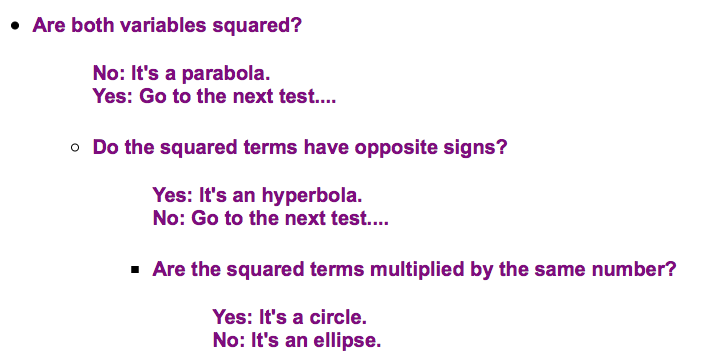
\includegraphics [scale=0.6] {conic_test.png} \end{center}

Kline goes through the effort of showing that, after rotating to a standard orientation, \emph{every} equation of the general form
\[ Ax^2 + Bxy + Cy^2 + Dx + Ey + F = 0 \]
can be translated to the origin to give a standard parabola, circle, ellipse or hyperbola.

\subsection*{conic sections}

\begin{center} 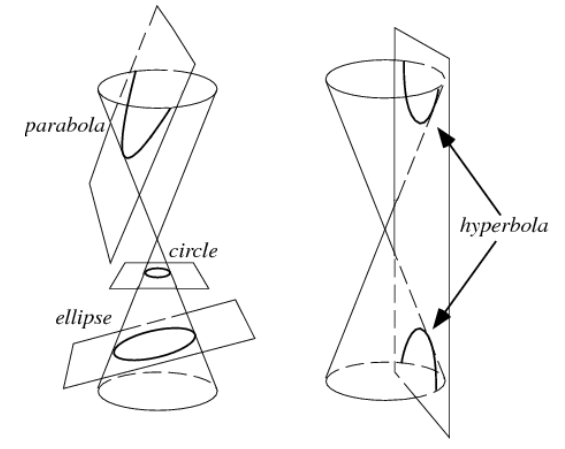
\includegraphics [scale=0.4] {conic_sections.png} \end{center}

Everyone learns in high school that the conic sections can be obtained by slicing a double cone with a plane and taking the points that belong to both.  Here is a simple example.

The level curves of a cone are
\[ x^2 + y^2 = r^2 \]
and the equation of the cone is $z = kr$ where $k = H/R$ is a constant.  Suppose $k = 1$.

Suppose we also have a plane like
\[ z = y + 1 \]
This plane has normal vector
\[ \mathbf{N} = \ \langle 0, -1, 1 \rangle \]
so the $x$-axis lies in the plane because $\mathbf{N} \cdot \mathbf{\hat{i}} = 0$.  Another vector orthogonal to both and also in the plane is $\langle 0, 1, 1 \rangle$.

The normal vector to the cone depends on where you are, but if you are at $x=0, y=1$ then it would be
\[ \mathbf{N} = \ \langle 0, 1, -1 \rangle \]
In the $yz$-plane it points down at a 45 degree angle.  The two normal vectors are the same (within sign), so if there is a solution it should be a parabola.

We can see that there should be a solution, because the plane intersects the $y$-axis at $y = -1$ ($z = 0$) and the $z$-axis at $z = 1$.  If you draw a sketch, one point is outside the cone and the other inside it, so the plane must cut the cone.

Every point on the intersection of the plane and the cone satisfies both equations:
\[ \sqrt{x^2 + y^2} = 1 + y \]
\[ x^2 + y^2 = 1 + 2y + y^2 \]
\[ x^2/2 = y + 1/2 \]

This is a parabola but it is \emph{not} the parabola formed by the intersection.  It is the projection of that intersection onto the $xy$-plane.

Such projections are linear transformations, which simply amount to rescaling of the variables $x$ to $x'$ and $y'$ to $y'$ (in this case only the latter) without changing the nature of the curve---a parabola is still a parabola.  

However, an ellipse may become a circle, and vice-versa.

In this case, the normal vector forms an angle of 45 degrees with the vertical $z$-axis since
\[ \cos \theta = \frac{\langle 0, -1, 1 \rangle \cdot \langle 0, 0, 1 \rangle}{\sqrt{1 + 1} \ \sqrt{1}} = \frac{1}{\sqrt{2}} \]
This is the factor by which the actual curve is stretched compared to the projection in the plane.

For the general problem, we would need to rotate all the points on the curve using angles obtained from the normal vector.  We want to tilt $\mathbf{N}$ so that it points straight up and has its magnitude unchanged.

\url{https://en.wikipedia.org/wiki/Rotation_matrix}

In 3D we we could rotate points (or the coordinate system) first with respect to the $xy$-plane (ignoring $z$) using the standard transformation with this matrix

\[
\begin{bmatrix}  
\cos \theta & -\sin \theta & 0 \\
\sin \theta & \ \  \cos \theta & 0 \\
0 & 0 & 1 
\end{bmatrix}
\begin{bmatrix}  x \\ y \\ z \end{bmatrix}
\]

This is the same rotation that we had before --- it leaves the $z$-coordinate unchanged.  The relevant $t$ is calculated from the $x$ and $y$ components of $\mathbf{N}$ using $t = \tan^{-1} y/x$.  Then use the given matrix, or perhaps switch the signs on the sine.

After $\mathbf{N}$ has been rotated so that it lies along either the $x$- or $y$-axis, then rotate in the $xz$-plane or $yz$-plane until N is vertical.

Having done this, I believe there should be no mixed terms containing $xy$, so we won't need to rotate to remove those, as done before.
 
\end{document}